\section{Compiler Overview}
\label{Sec:Overview}
\Treebeard{} takes a serialized decision tree ensemble as input (E.g.:
XGBoost JSON, ONNX etc.) and automatically generates an optimized inference function. 
\Treebeard{} automatically generates an optimized inference function from 
the serialized model and can either target CPUs or GPUs. 
Figure \ref{Fig:CompilerStructure} shows the structure of the \Treebeard{} compiler. 
The inference computation is lowered through three intermediate representations
-- high-level IR (HIR), mid-level IR (MIR) and low-level IR (LIR). The LIR is
finally lowered to LLVM and then JIT'ed to the specified target processor.

\begin{figure}[htb]
  \centering
  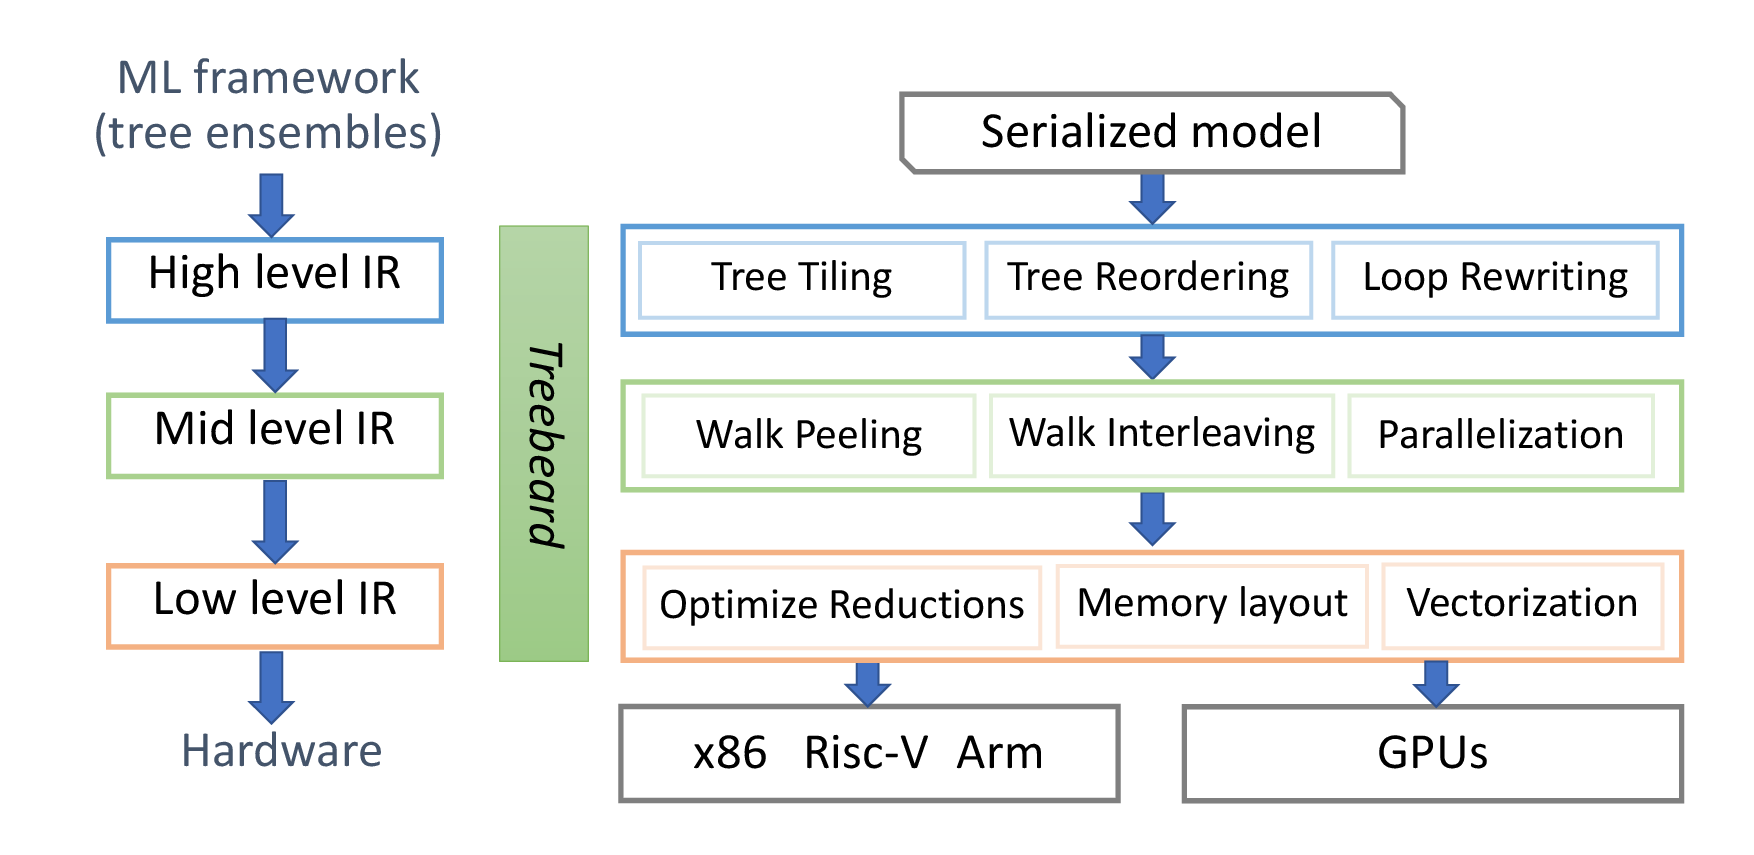
\includegraphics[width=\linewidth]{figures/compiler.png}
  \caption{\Treebeard{} compiler structure.}
  \label{Fig:CompilerStructure}
\end{figure}

\begin{figure}[htb]
  \centering
  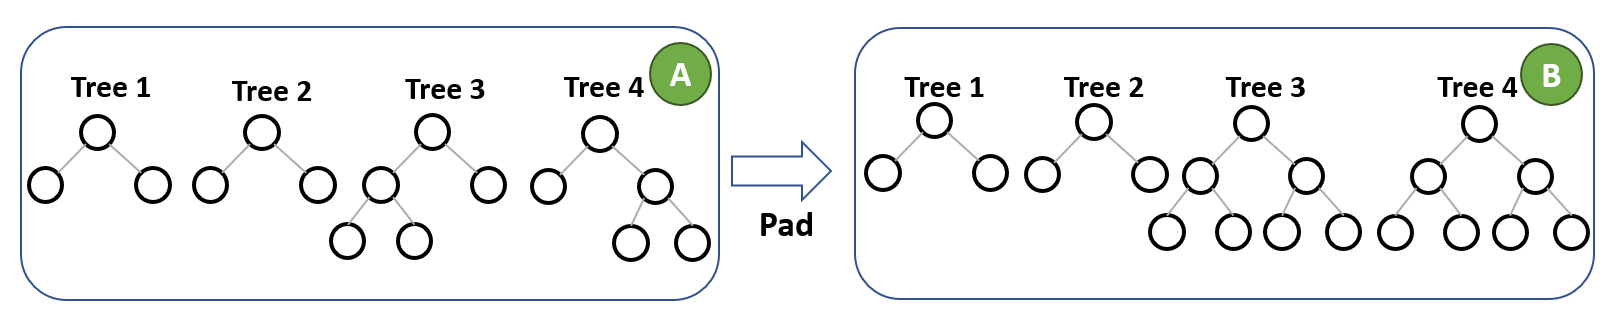
\includegraphics[width=\linewidth]{figures/HIR.PNG}
  \caption{The representation of a model in high-level IR and the model 
  after trees are padded and reordered. }
  \label{Fig:HIRExample}
\end{figure}

Table \ref{Tab:IRSpecification} lists the operations in the three IRs. 
In HIR, the model is represented as a collection of binary trees. This abstraction
allows the implementation of optimizations that require the manipulation of the model
or its constituent trees. Figure \ref{Fig:HIRExample} shows this representation for a model 
with four trees and how the model can be transformed. The model contains two trees of 
depth 1 and two trees of depth 2 (\circled{A}). The right side of the diagram shows the models after 
padding and reordering (\circled{B}). Padding makes all leaves in a tree the same depth (Trees 2 and
4 are padded). Trees are reordered so that trees of the same depth are together (Trees 
2 and 3 are swapped). We use this model as a running example for the rest of the section.
After these model-level optimizations are performed on the HIR, the 
code is lowered to the mid-level IR (MIR) as dictated by a  
\emph{\textbf{schedule}}. The schedule determines how to traverse
the iteration space that goes over the trees and input rows 
by specifying how loops are to be tiled, 
parallelized, mapped to GPU grid and block dimensions etc.
(Details in Section \ref{sec:schedule}). While MIR is a loop-based IR that 
explicitly encodes details of the iteration space has to be traversed, 
it still abstracts details about the in-memory representation of the model. 

In the lowered MIR, the compiler uses the \op{reduce} op from 
the \op{reduction} dialect we design (details in Section \ref{sec:reduction})
to represent reduction operations. The lowering of the \op{reduce} operation 
involves introducing temporary buffers and splitting the reduction 
to correctly implement reduction in the presence of 
parallel loops. This process, that we call \textbf{\emph{legalization}}, is 
described in Section \ref{sec:reduction}. 

The MIR is then further lowered to a low-level IR (LIR). This is the
level at which the compilation pipeline diverges for different targets. In 
the GPU compilation pipeline, the required memory transfers and kernel
invocations are inserted into the LIR. Additionally, buffers 
to hold model values are inserted and abstract tree operations are lowered to
explicitly refer to these buffers. This lowering is controlled by 
a plugin mechanism which enables different in-memory representations to 
be added to the compiler by implementing an interface 
(Section \ref{sec:representations}). Vectorization of tree traversals
is also explicitly represented in LIR.

In the remainder of this section, we show using our running example
from Figure \ref{Fig:HIRExample} how different schedules can be used to 
lower the model to MIR. We also show how the \op{reduce} operation
is lowered and legalized.

First, we consider the schedule that processes one tree at a time 
for all input rows and unrolls all tree walks. 
We assume that the trees have been reordered so that all trees with 
the same depth are together as shown in Figure \ref{Fig:HIRExample}.
The schedule splits the loop over the trees into two loops -- one that
iterates over the first two trees (Trees 1 and 3 with depth 1) and 
the second that iterates over the last two trees (Trees 2 and 4 with
depth 2). The schedule then unrolls the tree walks for each tree.
\begin{lstlisting}[style=c++]
  reorder(tree, batch)  
  split(tree, t0, t1, 2)
  unrollWalk(t0, 1)
  unrollWalk(t1, 2)
\end{lstlisting}

\Treebeard{} represents loops as nodes in a tree where the children
of a node represent immediately contained loops. Each schedule 
primitive modifies this tree in some way. For example, the \op{split}
primitive above duplicates the subtree rooted at the node that is 
being split. The compiler tracks the lineage of each of the loops. This allows 
the compiler to automatically infer the ranges for all loops. To lower the
HIR to MIR, the compiler traverses the tree of loops and generates the
appropriate loops. The MIR for the example model, generated using the above   
schedule is as follows. 
\begin{lstlisting}[style=c++]
  model = ensemble(...)
  for t0 = 0 to 2 step 1 {
    T = getTree(ensemble, t0)
    for batch = 0 to BATCH_SIZE step 1 {
      treePred = walkDecisionTree(T, 
                    input[batch]) <unrollDepth = 1>
      reduce(result[batch], treePred)
    }
  }
  for t1 = 2 to 4 step 1 {
    T = getTree(ensemble, t0)
    for batch = 0 to BATCH_SIZE step 1 {
      treePred = walkDecisionTree(T,
                    input[batch]) <unrollDepth = 2>
      reduce(result[batch], treePred) <'+', 0.0>
    }
  }
\end{lstlisting}
Subsequent lowering rewrites the \op{walkDecisionTree} operations to a 
series of \op{traverseTile} operations -- one for the 
first instance and two for the second (as specified by the unroll depth
attribute). \Treebeard{} also determines that the \op{reduce} operation
can be implemented by a simple addition operation as there are no 
surrounding parallel loops (The legalization of reductions is described 
in detail in Section \ref{sec:reduction}).

We now show how easily the same model can be compiled to target a GPU 
using \Treebeard{}'s scheduling language. 
A possible schedule to accomplish this is as follows.
\begin{lstlisting}[style=c++]
  tile(tree, t0, t1, 2)
  reorder(batch, t1, t0)
  split(t0, t0_1, t0_2, 2)
  unrollWalk(t0_1, 1)
  unrollWalk(t0_2, 2)
  gpuDimension(batch, grid.x)
  gpuDimension(t1, block.x)
\end{lstlisting}
This schedule processes one input row per thread block (since the \op{batch}
loop is mapped directly to \op{grid.x}).
It also splits the trees into two sets by tiling the \op{tree} loop.
Each of the two sets is processed in parallel. We unroll the tree walks 
for each tree. The MIR generated is as follows. 
\begin{lstlisting}[style=c++]
  model = ensemble(...)
  par.for batch = 0 to BATCH_SIZE step 1 <grid.x> {
    par.for t1 = 0 to 2 step 1 <block.x> {
      for t0_1 = 0 to 2 step 2 {
        T = getTree(ensemble, t0_1 + t1)
        treePred = walkDecisionTree(T, 
                        input[batch]) <unrollDepth = 1>
        reduce(result[batch], treePred)
      }
      for t0_2 = 2 to 4 step 2 {
        T = getTree(ensemble, t0_2 + t1)
        treePred = walkDecisionTree(T,
                        input[batch]) <unrollDepth = 2>
        reduce(result[batch], treePred) <'+', 0.0>
      }
    }
  }
\end{lstlisting}

In the case of this schedule, the lowering passes for the \op{reduce}
operation determines that parallel iterations of the \op{t1} 
loop accumulate into the same element of the \op{result} array.
Therefore, the reduction is rewritten so that each parallel 
iteration accumulates into a different array element by introducing 
a temporary buffer (\op{tempResults}) as follows.
\begin{lstlisting}[style=c++]
  float tempResults[2][BATCH_SIZE]
  model = ensemble(...)
  par.for batch = 0 to BATCH_SIZE step 1 <grid.x> {
    par.for t1 = 0 to 2 step 1 <block.x> {
      for t0_1 = 0 to 2 step 2 {
        T = getTree(ensemble, t0_1 + t1)
        treePred = walkDecisionTree(T, 
                      input[batch]) <unrollDepth = 1>
        reduce(tempResults[t1][batch], treePred)
      }
      for t0_2 = 2 to 4 step 2 {
        T = getTree(ensemble, t0_2 + t1)
        treePred = walkDecisionTree(T,
                      input[batch]) <unrollDepth = 2>
        reduce(tempResults[t1][batch], treePred) <'+', 0.0>
      }
    }
    result[batch] = reduce_dimension(tempResults[:][batch], 0)
  }
\end{lstlisting}
Here, partial results are accumulated into \op{tempResults} and then
reduced across the \op{t1} dimension (represented by the \op{reduce\_dimension}
operation) to get the final result. Finally, since this computation is 
being targeted to the GPU, the parallel loops are rewritten into kernel calls 
and the required GPU memory allocations and memory transfers are introduced.

As is evident from these examples, the structure of the loop 
nest in the inference routine can get quite complex even 
for simple schedules. Writing these routines by hand 
is error-prone and time-consuming. Building a principled code 
generator to automatically generate these routines is the 
best way to explore the vast design space. The key features in 
the design of \Treebeard{} that enable us to build such a code
generator are as follows.  

\begin{enumerate}
  \item The compiler uses three intermediate representations (IRs) to
  represent the inference computation at different levels of abstraction. This
  allows different optimizations to be performed and also allows us to share
  infrastructure between compilation pipelines for different target processors.

  \item The specification of how the inference computation is to be lowered to 
  loops is not encoded directly in the compiler. Instead, this 
  is specified as an input to the compiler using a scheduling language that is 
  specialized for decision tree inference computations (Section \ref{sec:schedule}).
  This separation allows us to build optimizations and schedule exploration 
  mechanisms independent of the core compiler (Section \ref{sec:exploring}). 

  \item \Treebeard{} has been designed to keep the optimization passes and code 
  generator independent of the in-memory representation finally used for the model. To achieve 
  this, \Treebeard{} specifies an interface to implement that provides the necessary 
  capabilities to the code generator as a plugin. This interface abstracts several details
  on how model values are stored (Details in Section \ref{sec:representations}). This 
  design allows us to write each in-memory representation as a standalone plugin 
  and reuse the rest of the compiler infrastructure. \TODO{Should we also say it lets us
  easily search over multiple representations?}
\end{enumerate}


%**************ROUGH*********************

% Another important 
% point to note is that MIR is independent of the target processor and therefore
% all optimizations on MIR can be reused across CPU and GPU compilation.


% \begin{figure*}[htb]
%   \centering
%   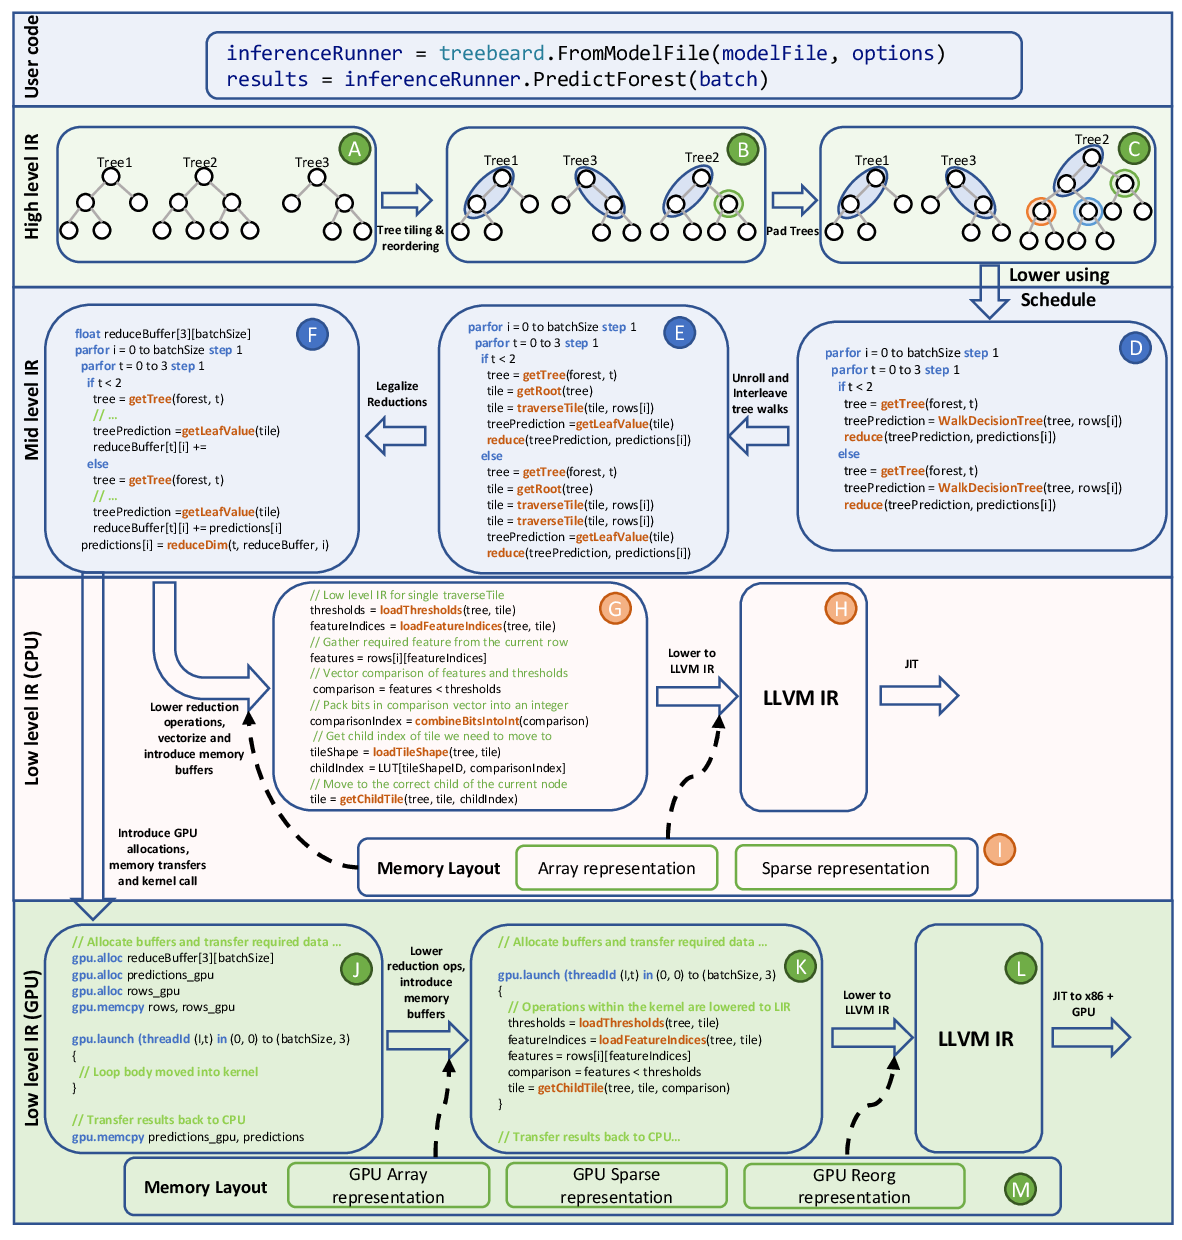
\includegraphics[width=\linewidth]{figures/OverviewExample_New.png}
%   \vskip 10pt
%   \caption{\Treebeard{} IR lowering and optimization details: the three abstraction levels in \Treebeard{}'s IR are shown. The
%            high level IR is a tree-based IR to perform model level optimization, the mid-level IR is for
%            loop optimizations that are independent of memory layout and the low level IR allows us to perform
%            vectorization and other memory layout dependent optimizations.}
%   \label{Fig:LoweringExample}
% \end{figure*}

% \begin{figure*}[htb]
%   \centering
%   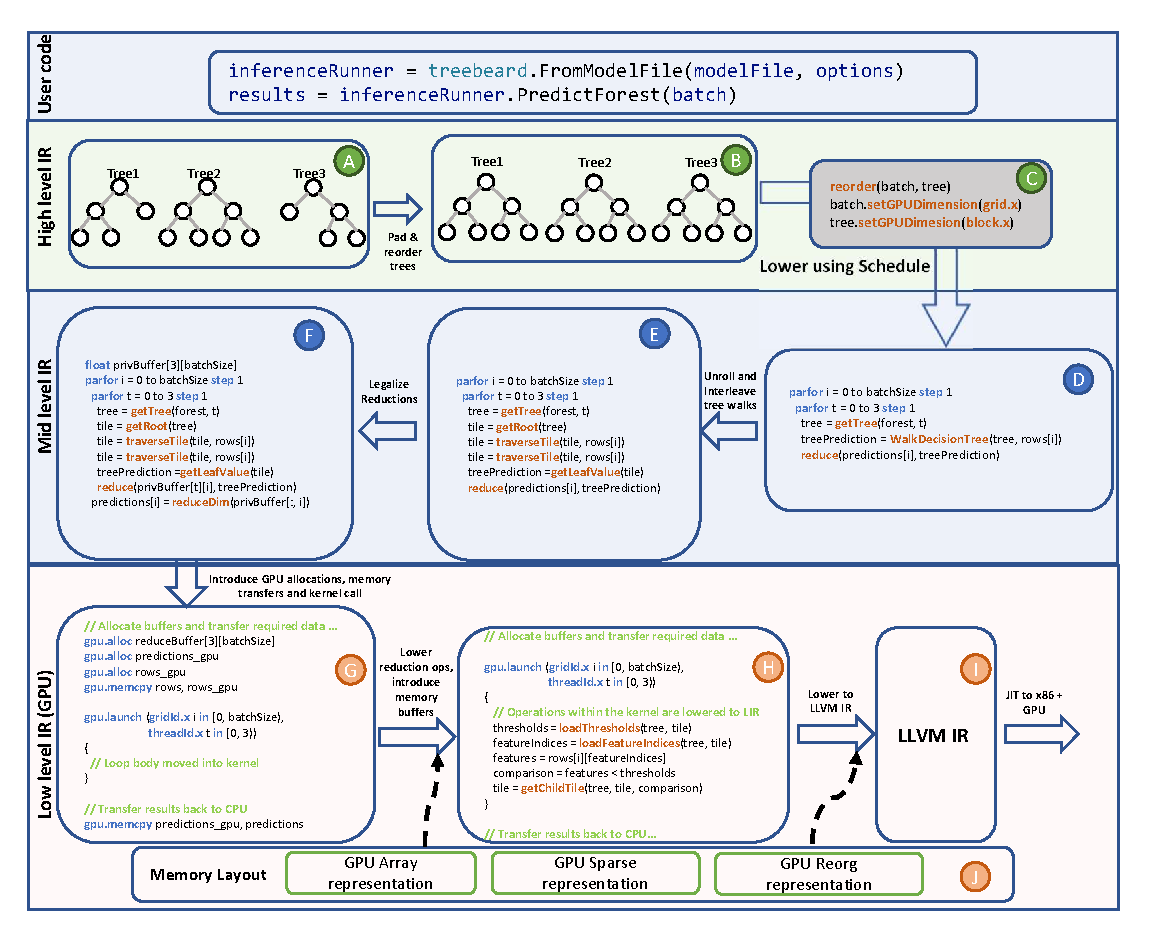
\includegraphics[width=\linewidth]{figures/GPUCompilationOverview-cropped.pdf}
%   \vskip 10pt
%   \caption{\Treebeard{} IR lowering and optimization details: the three abstraction levels in \Treebeard{}'s IR are shown. The
%            high level IR is a tree-based IR to perform model level optimization, the mid-level IR is for
%            loop optimizations that are independent of memory layout and the low level IR allows us to perform
%            vectorization and other memory layout dependent optimizations.}
%   \label{Fig:GPULoweringExample}
% \end{figure*}

% In HIR, the model is represented as a collection of binary trees. This abstraction
% allows the implementation of optimizations that require the manipulation of the model
% or its constituent trees. In Figure \ref{Fig:LoweringExample}, \circled{A}
% shows this representation for a model with three trees. 
% In HIR, \Treebeard{} tiles tree nodes together to convert
% the binary tree to an n-ary tree as shown in \circled{B}. Trees are also 
% reordered to enable better code generation and padded to allow more 
% efficient traversal as shown in \circled{C}. While these are the optimizations currently 
% implemented in \Treebeard{}, these are by no means the only ones that 
% are enabled by HIR. It is not difficult to imagine optimizations 
% such as tree pruning for specified accuracy levels for example.
% These optimizations and rewrites that are performed on the domain-specific 
% HIR would have been much on a traditional loop based IR or even in 
% other IRs within \Treebeard{}.


% After these model-level optimizations are performed on the HIR, the 
% code is lowered to the mid-level IR (MIR) as dictated by a user specified schedule
% (\circled{C} to \bluecircled{D}) in Figure \ref{Fig:LoweringExample}). The schedule specifies how
% the iteration space that goes over the trees and input rows is to be traversed. 
% It specifies how the iteration space is to be tiled, which loops are to be
% parallelized, which loops are to be mapped to GPU grid and block dimensions etc.
% (Details in Section \ref{Sec:SchedulingLang}). MIR is a loop-based IR that 
% explicitly encodes details of the iteration space has to be traversed. However, 
% it still abstracts details about the in-memory representation of the model. 
% Optimizations such as tree-walk unrolling and interleaving are performed 
% on the MIR (\bluecircled{E}). Subsequently, reduction operations are split and rewritten 
% to correctly and explicitly implement reduction in the presence of 
% parallel loops (\bluecircled{F}). More details of this process that we call 
% \emph{legalization} are in Section \ref{Sec:Reduction}. Another important 
% point to note is that MIR is independent of the target processor and therefore
% all optimizations on MIR can be reused across CPU and GPU compilation.

% The MIR is then further lowered to a low-level IR (LIR). This is the
% level at which the compilation pipeline diverges for CPUs and GPUs. In 
% the GPU compilation pipeline, the required memory transfers and kernel
% invocations are inserted into the LIR (\circled{J}). Additionally, buffers 
% to hold model values are inserted and tree operations are lowered to
% explicitly refer to these buffers. This lowering is controlled by 
% a plugin mechanism where different in-memory representations can 
% be added to the compiler by implementing an interface. These plugins
% provide information required for the lowering of MIR to LIR as well as 
% the lowering to LLVM IR as shown in Figure \ref{Fig:LoweringExample}.
% Again, a significant amount of code is shared between the
% CPU and GPU pipelines for representations that are common between them
% (Array and Sparse representations). Vectorization of tree traversals 
% is also explicitly represented in LIR.